\documentclass[11pt, oneside]{article} 
\usepackage{geometry}
\geometry{letterpaper} 
\usepackage{graphicx}
	
\usepackage{amssymb}
\usepackage{amsmath}
\usepackage{parskip}
\usepackage{color}
\usepackage{hyperref}

\graphicspath{{/Users/telliott/Github/precalculus/fig/}}
% \begin{center} \includegraphics [scale=0.4] {gauss3.png} \end{center}

\title{Area of a circle}
\date{}

\begin{document}
\maketitle
\Large  

- Albert Einstein

\begin{quote}Any fool can know.  The point is to understand.\end{quote}

In this first unit we will develop the most famous of Archimedes geometrical contributions, a theorem on the volume of the sphere.  

Before we get there we need to talk about circles (a topic to which he also contributed) and look at the volume of cones and pyramids.  These are topics in geometry that come  before the volume of the sphere.

\subsection*{area}

But even before that, we need a brief introduction to area and volume.  In geometry there are lines and curves and each of these has length.  

Figures in the plane have area:  triangles, squares and rectangles, and straight-sided polygons, so-called rectilinear figures.  But also, circles and ellipses and parabolas.  

Then there are solid figures, like cubes and pyramids, and cones and spheres, that have volume.

For a rectangular figure, it is easy to see why the definition of area as length times  width makes sense.  For a cube, the volume is the length times width times height.  

One of the miracles of calculus is that it can give us areas and volumes of curved figures.  But some of those results were available from Greek geometry, even before calculus.  We'll see a bit of that here.  As we start reasoning about circles, we recognize that the area of a circle is going to be something \emph{squared}, because it occupies space in the plane.

According to wikipedia

\url{https://en.wikipedia.org/wiki/Area_of_a_circle}

Eudoxus of Cnidus, born in the 5th century (408 BCE), proved that the area of a circle, like that of regular polygons, is proportional to both horizontal and vertical dimensions, and thus is proportional to the radius squared.

An idea that I bet you've run into, and we will use a lot, is that the area of a triangle is one-half the base times the height.  This is easy to prove.  Here we show only an acute triangle, but the theorem is true for all:  any triangle can be divided into two right triangles.
\begin{center}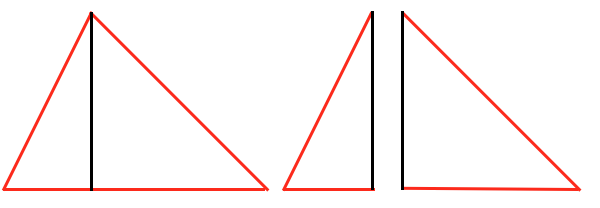
\includegraphics [scale=0.4] {area_triangle_1.png}\end{center}

The two pieces can then be pasted to their rotated equals to form two rectangles.
\begin{center}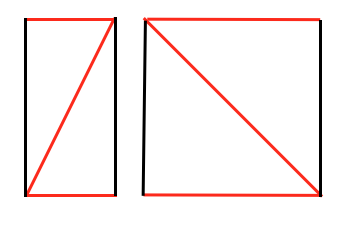
\includegraphics [scale=0.4] {area_triangle_2.png}\end{center}

The total area of each rectangle is the total base times the height.  The total area is the total base times the same height.  This is twice the area of the original triangle.

$\square$

\subsection*{circumference}

We move on to the circle.  A fundamental result about circles is that the ratio of the circumference of a circle to its diameter is independent of the size of the circle.  All circles have the same shape.
\begin{center}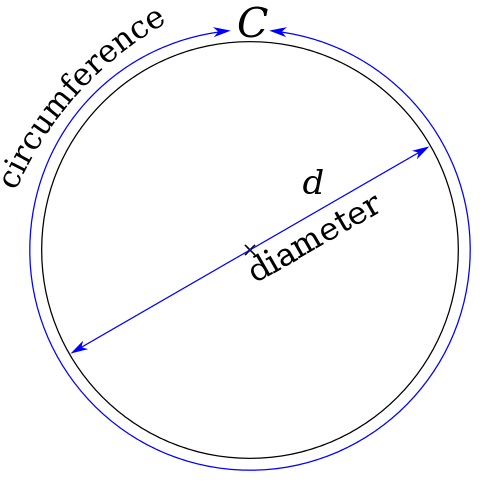
\includegraphics [scale=0.4] {circle0.png}\end{center}

The proportionality constant was named in the early 1700s and popularized by Euler a few decades later: 
\[ \pi = \frac{C}{d} \]
Since the radius is one-half the diameter, $2r = d$ and
\[ 2 \pi r = C \]

This is usually stated as a self-evident fact, but it is actually a theorem to be proved.  We defer that one for the moment.

\subsection*{area of a circle:  pizza proof}

Imagine dividing a circle into wedges, like you might do with a pizza.  Here, the pie has been divided into 16 parts.
\begin{center}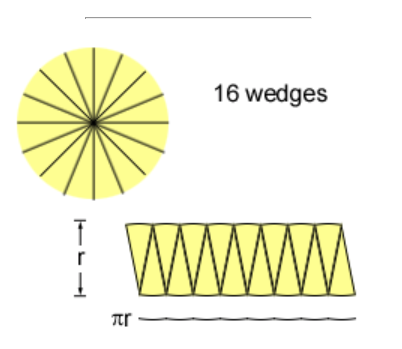
\includegraphics [scale=0.5] {circle_wedges.png}\end{center}

Since the pieces are triangular, it is easy to stack them next to each other with the bases and tips alternating, as shown.  Of course the bases are not straight, but have the same curvature as the edge of the circle.  

The length of the short side is the radius, $r$, although it is angled.  The original perimeter or circumference is divided into the top and the bottom of the figure, so the length of the long side is approximately one-half the circumference and thus, with length times width, we obtain
\[ A =  r\cdot \frac{1}{2} \cdot 2 \pi r = \pi r^2 \]

The trick is to imagine what happens if we subdivide the circle into many slices.  The more slices, the more vertical the side, and the straighter the edges.  If there are infinitely many  slices, the edges will be perfectly straight and this calculation becomes exact.

The pizza proof is very much like one attributed to Leonardo da Vinci, among others.

\subsection*{concentric rings}

Another idea is to remove concentric strips from the edge and stack them.
\begin{center}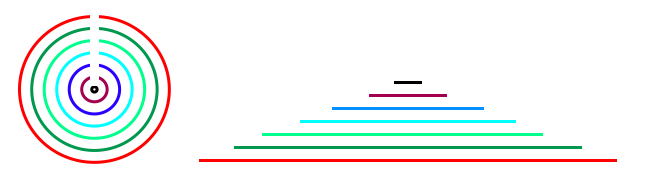
\includegraphics [scale=0.5] {circle_strips.png}\end{center}

This is actually the same calculation as we did previously, just based on a different idea.  Here, we imagine the concentric strips infinitely thin.

We obtain a triangle of height $r$ and base $2 \pi r$ so its area is
\[ \frac{1}{2} \ 2 \pi r \cdot r = \pi r^2 \]

\subsection*{concentric rings}

A formal proof that this triangle has the same area as the circle was given by Archimedes and is found in his \emph{Measurement of a Circle}, proposition 1.  However, many sources, including

\url{http://www.math.tamu.edu/~dallen/masters/Greek/eudoxus.pdf}

attribute the proof to Eudoxus, who was perhaps the second most famous mathematician of antiquity, and a colleague of Plato in Athens.

I love the proof, but some people have struggled with it, especially so early in the book.  If you struggle, just move on.  But please take a shot at it first.

We will sketch the idea and discuss it more formally \hyperref[sec:circle_proof]{\textbf{here}}.

The method used is called proof by contradiction, \emph{reductio ad absurdum}, which Hardy called

\begin{quote}one of the mathematicians finest weapons\end{quote}

One begins with an assumption.  A slightly strained analogy might be, turning into a narrow street and, having missed the sign, assuming it goes your way.  Later, when you meet a semi trailer head-on you know there is a problem somewhere in the logic.

\subsection*{inscribed polygon}
Draw a circle.  Call the actual, correct, yet still unknown value for the area of the circle $A$.

The idea is to draw a regular polygon (all sides equal length) inside the circle.  
\begin{center}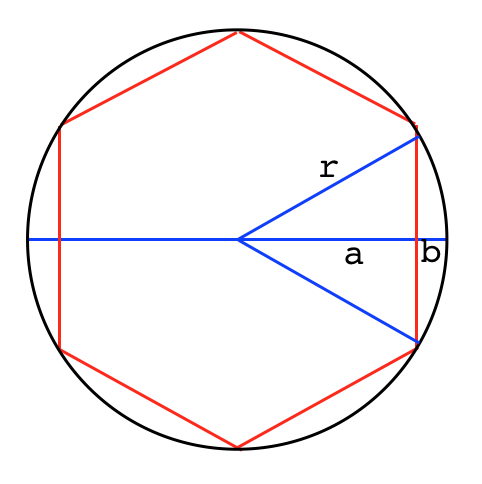
\includegraphics [scale=0.4] {area_circle_0.png}\end{center}

Here we have drawn a hexagon (6-sides).  If the lines from the center to the vertices have length $r$, then they divide the hexagon into six triangles, each with height $a$ and base length $b$, where $a < r$ and $b$ is less than the arc length.  Clearly the area of the triangle is less than the area of that sector of the circle.

The base of the triangle is closest to the center (and farthest from the edge) at the center of the base, where the line segment from the center is called the apothem (labeled $a$).  Using trigonometry, it isn't hard to calculate the area of the polygon, but we don't need to.  Just call it $P$.

\begin{center}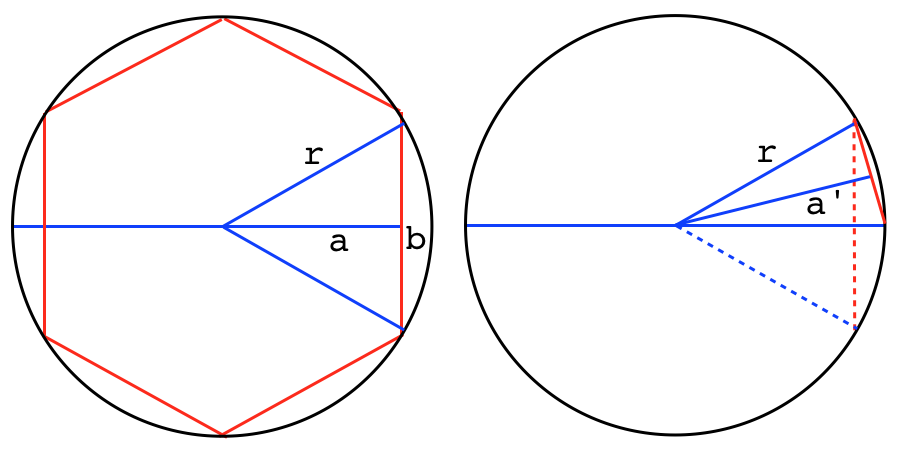
\includegraphics [scale=0.4] {area_circle_1.png}\end{center}

Archimedes now says, let us double the number of sides (right panel).  What happens then?

The new 12-sided polygon and its component triangles will have a larger apothem $a'$, and the total of all the bases all the way around will be larger and closer to the true circumference of the circle.  There is obviously less white space between the triangle's base and the perimeter of the circle.

Thus the new $P$ will be larger, and closer to $A$.

This doubling trick is easy to do.  We don't even have to carry it out, just imagine doing so.  We can make the difference between the area of the polygon $P$ and the circle's true area $A$ as as small as you please.  

If your boss decides it's not close enough, just double the number of sides \emph{again}.

That was all setup, here is the punchline.

\subsection*{proof}

Archimedes says, let us suppose that the true area of the circle $A$ is \emph{not} actually equal to $T$ (which is exactly $\pi r^2$) but is larger.  Just suppose.  In symbols, we are assuming that
\[ T < A \]

We've already seen that $P < A$

We know we can make $P$ as close to $A$ as we please.  

And therefore (the key point) we can make P \emph{closer} to $A$ than $T$ is.  The meaning of $T < A$ is that there must be some daylight between $T$ and $A$.  The side-doubling operation can get us into that window.

So now, by doubling, we have obtained a new $P$ that is larger than $T$.  We have established that
\[ T < P < A \]
If $T < A$ there is really no other choice.

But look at the figure below.  No matter how many sides our many-sided polygon has, $a < r$ and and the base must be less than the circumference of the circle so clearly $P < T$ for any polygon.
\begin{center}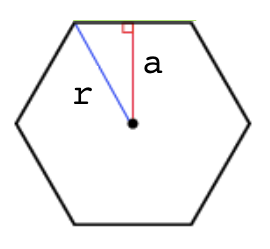
\includegraphics [scale=0.5] {apothem2.png}\end{center}

This is a contradiction.  We have shown by two arguments which are both logically correct that $P < T$ and also that $P > T$.  There is something wrong.

The resolution is that assumption we made above, that $A > T$, cannot be right.  Therein lies our problem.  $A$ is not greater than $T$.  It is either less than or equal to $T$.

But now try it the other way around. Circumscribe the circle with a hexagon that goes around the outside and run the argument again, and you will find that it cannot be true that $A < T$ either.

But if $A$ is neither less than nor greater than $T$ there is only one possibility, equality:
\[ A = T = \pi r^2 \]

$\square$

Plutarch, talking about Archimedes:

\begin{quote}It is not possible to find in all geometry more difficult and intricate questions, or more simple and lucid explanations. Some ascribe this to his natural genius; while others think that incredible effort and toil produced these, to all appearances, easy and unlabored results. No amount of investigation of yours would succeed in attaining the proof, and yet, once seen, you immediately believe you would have discovered it; by so smooth and so rapid a path he leads you to the conclusion required.\end{quote}

There is one additional point.  Archimedes actually provides a way of calculating the improved area of each successive polygon (or its perimeter, it is really the same problem) obtained by side-doubling.

Each cycle gives a smaller and smaller improvement, which means that there is a limiting value of this process.

That value is $\pi$, when talking about the perimeter for a unit diameter, or equivalently  when talking about the area, for a unit radius.  We will see how this works later, suffice it to say that the side-doubling trick gives us a way to calculate the value of $\pi$ to any accuracy we have the patience to compute.

\end{document}